%%%%%%%%%%%%%%%%%%%%%%%%%%%%%%%%%%%%%%%%%
% Masters/Doctoral Thesis 
% LaTeX Template
% Version 2.5 (27/8/17)
%
% This template was downloaded from:
% http://www.LaTeXTemplates.com
%
% Version 2.x major modifications by:
% Vel (vel@latextemplates.com)
%
% This template is based on a template by:
% Steve Gunn (http://users.ecs.soton.ac.uk/srg/softwaretools/document/templates/)
% Sunil Patel (http://www.sunilpatel.co.uk/thesis-template/)
%
% Template license:
% CC BY-NC-SA 3.0 (http://creativecommons.org/licenses/by-nc-sa/3.0/)
%
%%%%%%%%%%%%%%%%%%%%%%%%%%%%%%%%%%%%%%%%%

%----------------------------------------------------------------------------------------
%	PACKAGES AND OTHER DOCUMENT CONFIGURATIONS
%----------------------------------------------------------------------------------------

\documentclass[
11pt, % The default document font size, options: 10pt, 11pt, 12pt
oneside, % Two side (alternating margins) for binding by default, uncomment to switch to one side
spanish, % ngerman for German
singlespacing, % Single line spacing, alternatives: onehalfspacing or doublespacing
%draft, % Uncomment to enable draft mode (no pictures, no links, overfull hboxes indicated)
%nolistspacing, % If the document is onehalfspacing or doublespacing, uncomment this to set spacing in lists to single
%liststotoc, % Uncomment to add the list of figures/tables/etc to the table of contents
%toctotoc, % Uncomment to add the main table of contents to the table of contents
%parskip, % Uncomment to add space between paragraphs
%nohyperref, % Uncomment to not load the hyperref package
headsepline, % Uncomment to get a line under the header
%chapterinoneline, % Uncomment to place the chapter title next to the number on one line
%consistentlayout, % Uncomment to change the layout of the declaration, abstract and acknowledgements pages to match the default layout
]{MastersDoctoralThesis} % The class file specifying the document structure

\usepackage[utf8]{inputenc} % Required for inputting international characters
\usepackage[T1]{fontenc} % Output font encoding for international characters

\usepackage{placeins}
\usepackage{listings}

\usepackage{verbatim} % Comments: \begin{ comment } ... \end{ ... }

\newcommand{\keyword}[1]{\textbf{#1}}
\newcommand{\tabhead}[1]{\textbf{#1}}
\newcommand{\code}[1]{\texttt{#1}}
\newcommand{\file}[1]{\texttt{\bfseries#1}}
\newcommand{\option}[1]{\texttt{\itshape#1}}

\lstset{literate=
	{á}{{\'a}}1 {é}{{\'e}}1 {í}{{\'i}}1 {ó}{{\'o}}1 {ú}{{\'u}}1
	{Á}{{\'A}}1 {É}{{\'E}}1 {Í}{{\'I}}1 {Ó}{{\'O}}1 {Ú}{{\'U}}1
	{à}{{\`a}}1 {è}{{\`e}}1 {ì}{{\`i}}1 {ò}{{\`o}}1 {ù}{{\`u}}1
	{À}{{\`A}}1 {È}{{\'E}}1 {Ì}{{\`I}}1 {Ò}{{\`O}}1 {Ù}{{\`U}}1
	{ä}{{\"a}}1 {ë}{{\"e}}1 {ï}{{\"i}}1 {ö}{{\"o}}1 {ü}{{\"u}}1
	{Ä}{{\"A}}1 {Ë}{{\"E}}1 {Ï}{{\"I}}1 {Ö}{{\"O}}1 {Ü}{{\"U}}1
	{â}{{\^a}}1 {ê}{{\^e}}1 {î}{{\^i}}1 {ô}{{\^o}}1 {û}{{\^u}}1
	{Â}{{\^A}}1 {Ê}{{\^E}}1 {Î}{{\^I}}1 {Ô}{{\^O}}1 {Û}{{\^U}}1
	{œ}{{\oe}}1 {Œ}{{\OE}}1 {æ}{{\ae}}1 {Æ}{{\AE}}1 {ß}{{\ss}}1
	{ű}{{\H{u}}}1 {Ű}{{\H{U}}}1 {ő}{{\H{o}}}1 {Ő}{{\H{O}}}1
	{ç}{{\c c}}1 {Ç}{{\c C}}1 {ø}{{\o}}1 {å}{{\r a}}1 {Å}{{\r A}}1
	{€}{{\euro}}1 {£}{{\pounds}}1 {«}{{\guillemotleft}}1
	{»}{{\guillemotright}}1 {ñ}{{\~n}}1 {Ñ}{{\~N}}1 {¿}{{?`}}1
}

%\usepackage{mathpazo} % Use the Palatino font by default

\usepackage[backend=bibtex,style=numeric,natbib=true]{biblatex} % Use the bibtex backend with the authoryear citation style (which resembles APA)

\addbibresource{example.bib} % The filename of the bibliography

\usepackage[autostyle=true]{csquotes} % Required to generate language-dependent quotes in the bibliography

%----------------------------------------------------------------------------------------
%	MARGIN SETTINGS
%----------------------------------------------------------------------------------------

\geometry{
	paper=a4paper, % Change to letterpaper for US letter
	inner=2.5cm, % Inner margin
	outer=3.8cm, % Outer margin
	bindingoffset=.5cm, % Binding offset
	top=1.5cm, % Top margin
	bottom=1.5cm, % Bottom margin
	%showframe, % Uncomment to show how the type block is set on the page
}

%----------------------------------------------------------------------------------------
%	THESIS INFORMATION
%----------------------------------------------------------------------------------------

\thesistitle{Propuesta t\'ecnica y econ\'omica} % Your thesis title, this is used in the title and abstract, print it elsewhere with \ttitle
\supervisor{721556\\716205\\718997\\721288\\566416\\718123\\715750} % Your supervisor's name, this is used in the title page, print it elsewhere with \supname
\examiner{} % Your examiner's name, this is not currently used anywhere in the template, print it elsewhere with \examname
\degree{} % Your degree name, this is used in the title page and abstract, print it elsewhere with \degreename
\author{Jorge Aznar L\'opez\\Ángel Cañal Muniesa\\Abel Chils Trabanco\\Yasmina Albero Escudero\\\'Oscar Fraca Ferr\'andez\\Alexandru Ioan Oarga Hategan\\Jorge Pinilla López} % Your name, this is used in the title page and abstract, print it elsewhere with \authorname
\addresses{} % Your address, this is not currently used anywhere in the template, print it elsewhere with \addressname

\subject{Trabajo de la asignatura} % Your subject area, this is not currently used anywhere in the template, print it elsewhere with \subjectname
\keywords{} % Keywords for your thesis, this is not currently used anywhere in the template, print it elsewhere with \keywordnames
\university{\href{http://www.unizar.es}{Universidad de Zaragoza}} % Your university's name and URL, this is used in the title page and abstract, print it elsewhere with \univname
\department{\href{http://eina.unizar.es}{Escuela de Ingeniería y Arquitectura}} % Your department's name and URL, this is used in the title page and abstract, print it elsewhere with \deptname
\group{\href{http://researchgroup.university.com}{Research Group Name}} % Your research group's name and URL, this is used in the title page, print it elsewhere with \groupname
\faculty{\href{http://faculty.university.com}{Faculty Name}} % Your faculty's name and URL, this is used in the title page and abstract, print it elsewhere with \facname

\AtBeginDocument{
\hypersetup{pdftitle=\ttitle} % Set the PDF's title to your title
\hypersetup{pdfauthor=\authorname} % Set the PDF's author to your name
\hypersetup{pdfkeywords=\keywordnames} % Set the PDF's keywords to your keywords
}

\begin{document}

\frontmatter % Use roman page numbering style (i, ii, iii, iv...) for the pre-content pages

\pagestyle{plain} % Default to the plain heading style until the thesis style is called for the body content

%----------------------------------------------------------------------------------------
%	TITLE PAGE
%----------------------------------------------------------------------------------------

\begin{titlepage}
	\begin{center}
		
		\vspace*{.06\textheight}
		{\scshape\LARGE \univname\par}\vspace{1.5cm} % University name
		\textsc{\Large \subjectname}\\[0.5cm] % Thesis type
		
		\HRule \\[0.4cm] % Horizontal line
		{\huge \bfseries \ttitle\par}\vspace{0.4cm} % Thesis title
		\HRule \\[1.5cm] % Horizontal line
		
		\begin{minipage}[t]{0.4\textwidth}
			\begin{flushleft} \large
				\emph{Autor/es:}\\
				\authorname % Author name - remove the \href bracket to remove the link
			\end{flushleft}
		\end{minipage}
		\begin{minipage}[t]{0.4\textwidth}
			\begin{flushright} \large
				\emph{NIA/s} \\
				\supname % Supervisor name - remove the \href bracket to remove the link  
			\end{flushright}
		\end{minipage}\\[3cm]
		
		\vfill
		
		%{
\includegraphics{Figures/logo-eina.png}}\\ % University/department logo - uncomment to place it
		%\large \textit{A thesis submitted in fulfillment of the requirements\\ for the degree of \degreename}\\[0.3cm] % University requirement text
		%\textit{in the}\\[0.4cm]
		%\groupname\\\deptname\\[2cm] % Research group name and department name
		
		\vspace{5cm}
		\vfill
		
\includegraphics{Figures/logo-eina.png}\\ % University/department logo - uncomment to place it
		{\large \today}\\[4cm] % Date
		
		\vfill
	\end{center}
\end{titlepage}

%----------------------------------------------------------------------------------------
%	DECLARATION PAGE
%----------------------------------------------------------------------------------------
\begin{comment}
\begin{declaration}
\addchaptertocentry{\authorshipname} % Add the declaration to the table of contents
\noindent I, \authorname, declare that this thesis titled, \enquote{\ttitle} and the work presented in it are my own. I confirm that:

\begin{itemize} 
\item This work was done wholly or mainly while in candidature for a research degree at this University.
\item Where any part of this thesis has previously been submitted for a degree or any other qualification at this University or any other institution, this has been clearly stated.
\item Where I have consulted the published work of others, this is always clearly attributed.
\item Where I have quoted from the work of others, the source is always given. With the exception of such quotations, this thesis is entirely my own work.
\item I have acknowledged all main sources of help.
\item Where the thesis is based on work done by myself jointly with others, I have made clear exactly what was done by others and what I have contributed myself.\\
\end{itemize}
 
\end{declaration}

\cleardoublepage
\end{comment}
%----------------------------------------------------------------------------------------
%	QUOTATION PAGE
%----------------------------------------------------------------------------------------
\begin{comment}
\vspace*{0.2\textheight}

\noindent\enquote{\itshape Thanks to my solid academic training, today I can write hundreds of words on virtually any topic without possessing a shred of information, which is how I got a good job in journalism.}\bigbreak

\hfill Dave Barry
\end{comment}
%----------------------------------------------------------------------------------------
%	ABSTRACT PAGE
%----------------------------------------------------------------------------------------
\begin{comment}
\begin{abstract}
\addchaptertocentry{\abstractname} % Add the abstract to the table of contents
The Thesis Abstract is written here (and usually kept to just this page). The page is kept centered vertically so can expand into the blank space above the title too\ldots
\end{abstract}
\end{comment}
%----------------------------------------------------------------------------------------
%	LIST OF CONTENTS/FIGURES/TABLES PAGES
%----------------------------------------------------------------------------------------

\tableofcontents % Prints the main table of contents

%\listoffigures % Prints the list of figures

%\listoftables % Prints the list of tables

%----------------------------------------------------------------------------------------
%	DEDICATION
%----------------------------------------------------------------------------------------

% \dedicatory{For/Dedicated to/To my\ldots} 

%----------------------------------------------------------------------------------------
%	THESIS CONTENT - CHAPTERS
%----------------------------------------------------------------------------------------

\mainmatter % Begin numeric (1,2,3...) page numbering

\pagestyle{thesis} % Return the page headers back to the "thesis" style

% Include the chapters of the thesis as separate files from the Chapters folder
% Uncomment the lines as you write the chapters

% Chapter Template

\chapter{Resumen Ejecutivo} % Main chapter title

\label{Chapter1} % Change X to a consecutive number; for referencing this chapter elsewhere, use \ref{ChapterX}

%----------------------------------------------------------------------------------------
%	SECTION 1
%----------------------------------------------------------------------------------------

\section{Resumen}

La aplicación a desarrollar consistirá en un repositorio de música. 

Algunas consideraciones:
\begin{itemize}
	\item El resumen debe caber en una página, salvo que incluya algún gráfico o diagrama.
	\item Se debe incluir un resumen del sistema a desarrollar. Se puede partir de la propia descripción que nos haya dado el cliente.
	\item Se deben incluir el precio, los plazos y los entregables.
\end{itemize}

% Chapter Template

\chapter{Objetivos del sistema} % Main chapter title

\label{Chapter2} % Change X to a consecutive number; for referencing this chapter elsewhere, use \ref{ChapterX}

%----------------------------------------------------------------------------------------
%	SECTION 1
%----------------------------------------------------------------------------------------

\section{Objetivos}

Para la creación de contenido se permite el registro. Se contará con tanto con 3 perfiles de usuario: sin registro, con registro y administrador.
La aplicación cuenta a su vez con una version de Web y una version movil para Android con reproducción sincronizada entre ambos.
Los usuarios registrados tienen la posibilidad de administrar listas de reproducción públicas o privadas y a su vez el sistema genera listas de recomendaciones generales y para cada ususario.
A continuación se detalla el total de los requisitos.

\subsection{An\'alisis de requisitos preliminar}

\begin{itemize}
\item La aplicación permite reproducir canciones almacenadas en el repositorio.
\item La aplicación tendrá una versión para Android y otra para Web.
\item Existen 3 perfiles de usuario: registrados, no registrados y administrador.
\item Los usuarios registrados pueden generar y consumir contenido (canciones).
\item Los usuario no registrados solo pueden consumir contenido en la Web.
\item El sistema permite gestionar listas de reproducción públicas y privadas.
\item Se permite el login con la cuenta de usuario o con una cuenta Google mediante OAuth.
\item Verificación de cuenta. Esto supone un indicador gráfico en el perfil de usuario que anteriormente a verificado su identidad. La finalidad es garantizar la verdadera identidad del usuario.
\item En la versión movil, se permite almacenar la música en el dispositivo para poder acceder a esta sin conexión a internet.
\item La reproducción actual de un usuario se sincroniza en todos los dispositivos.
\item Integración con redes sociales, con la finalidad de compartir música, listas o perfiles en las RRSS.
\item Permite al usuario registrado generar sus propias listas de reproducción.

\item Un usuario registrado puede seleccionar 'Me gusta' en una canción.
\item Un usuario registrado puede suscribirse a otro usuario.
\item El sistema genera listas de reproducción segun las siguientes categorias: Género, Éxitos, Situación/Mood, País.
\item El sistema genera listas de reproduccion propias para cada usuario con recomendaciones según sus intereses.
\item El sistema genera listas de reproduccion con recomendaciones según geolocalización.
\item El sistema permite gestionar una lista privada de favoritos.
\item El sistema permite la búsqueda de canciones, albumes, listas y artistas.
\item El usuario administrador se utiliza para verificar, añadir o eliminar cuentas de usuarios.

\item Existe un servidor para el almacenamiento de canciones.
\item Los datos que se recogen en el formulario de registro son los siguientes: Nombre, Nick, Correo, Contraseña, Fecha de nacimiento, Biografía, Redes Sociales, Foto de perfil(opcional), País
\item Las canciones contienen los siguientes metadatos: Título, Idioma (opcional), número de reproducciones, número de 'Me gusta'.
\item La aplicación movil soportará Android 5.0
\item El sistema soporta los ficheros MP3, WAV, OGG.
\item La aplicación movil soporta la última versión de Firefox y Chrome.
\item El acceso al servidor se realiza a través de una API REST.
\end{itemize}

\subsection{Prototipo pantallas Android}
% ______________________
% Aqui comienza la tabla
\begin{tabular}{ p{6cm} p{6cm}}
\hline
\\
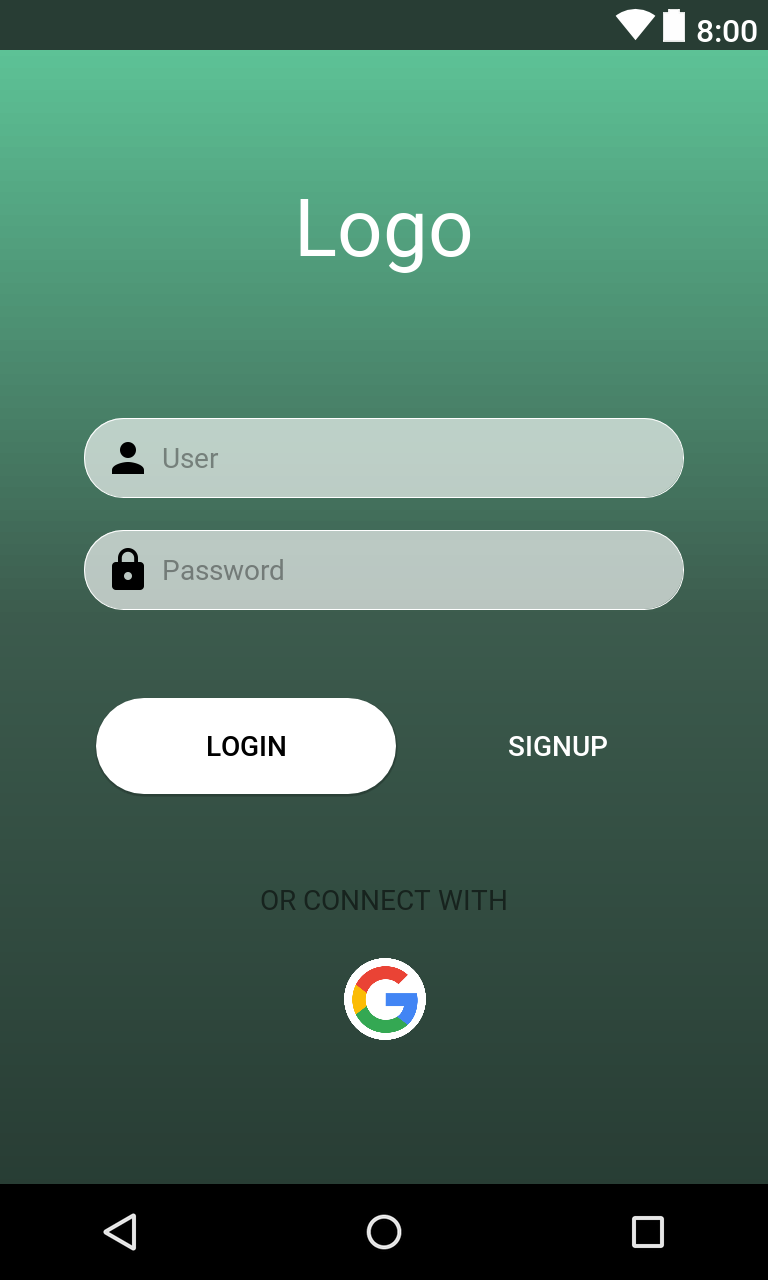
\includegraphics[width=6cm]{Figures/android/Login.png}
&
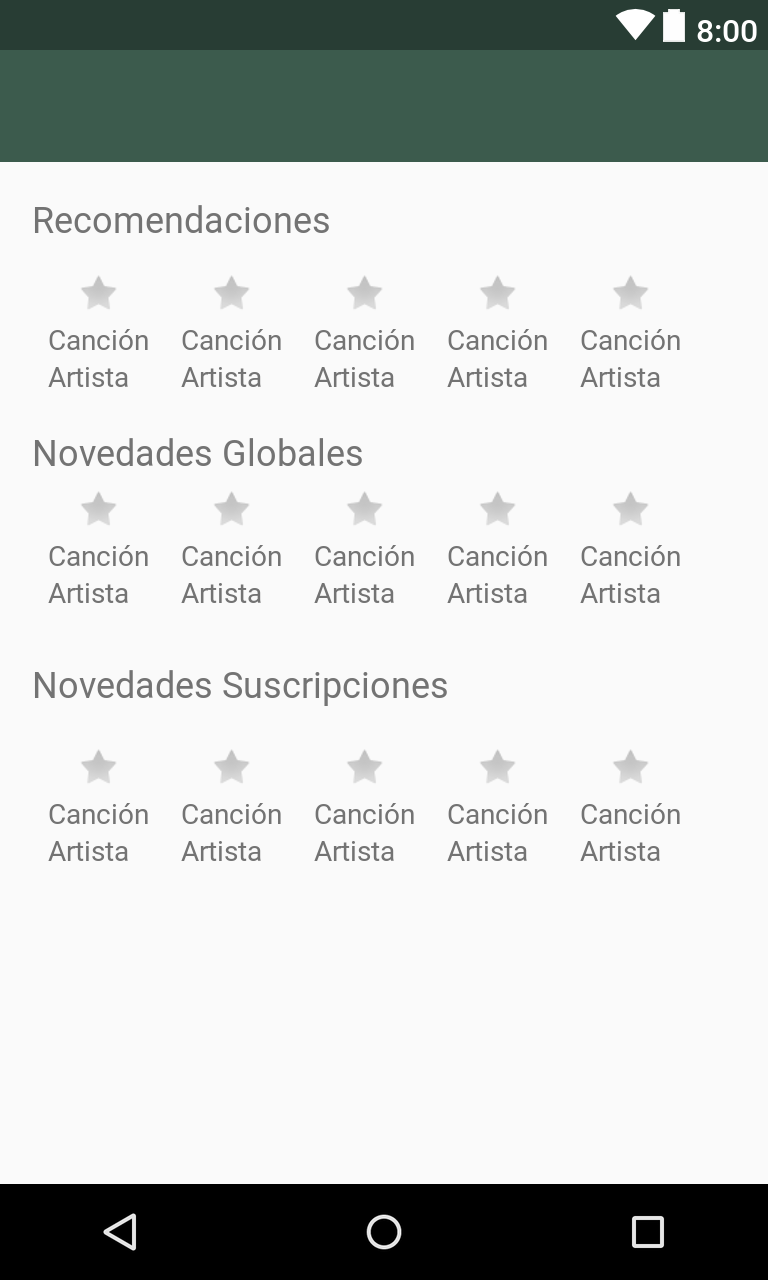
\includegraphics[width=6cm]{Figures/android/home.png} \\
\hline
\\
Pantalla de autentificación, en la que se permite tanto el acceso desde un usuario y contraseña de la aplicación así como desde una cuenta de Google. Esta es la primera pantalla que se abre en el caso de que el usuario no esté conectado
&
Pantalla principal de la aplicación en la cual se mostrarían diversos elementos de interés para el usuario, como pueden ser recomendaciones, novedades así como nuevas publicaciones que han producido artistas a los que se está suscrito.
Este esquema de pantalla también lo comparte una pantalla llamada explorar, la pantalla de novedades y la pantalla de recomendaciones.
En la pantalla explorar se mostrarían diversas listas de reproducción generadas por el sistema ( listas basadas en la ubicación del usuario, basadas en lo que escucha el usuario, basadas en lo que escucha el conjunto total de usuarios) así como los diferentes géneros musicales.  \\
\hline
\end{tabular}

\begin{tabular}{ p{6cm} p{6cm}}
\hline
\\
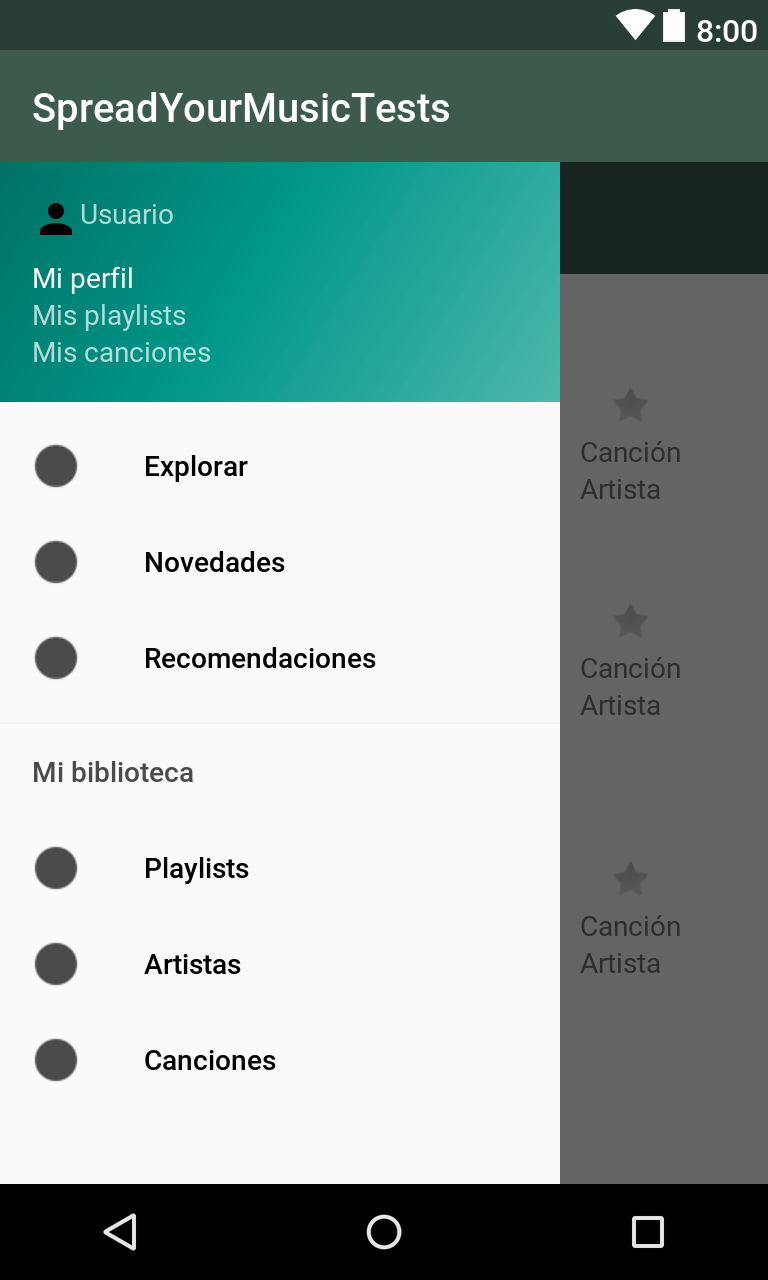
\includegraphics[width=6cm]{Figures/android/Home-NavigationDrawer.png}
&
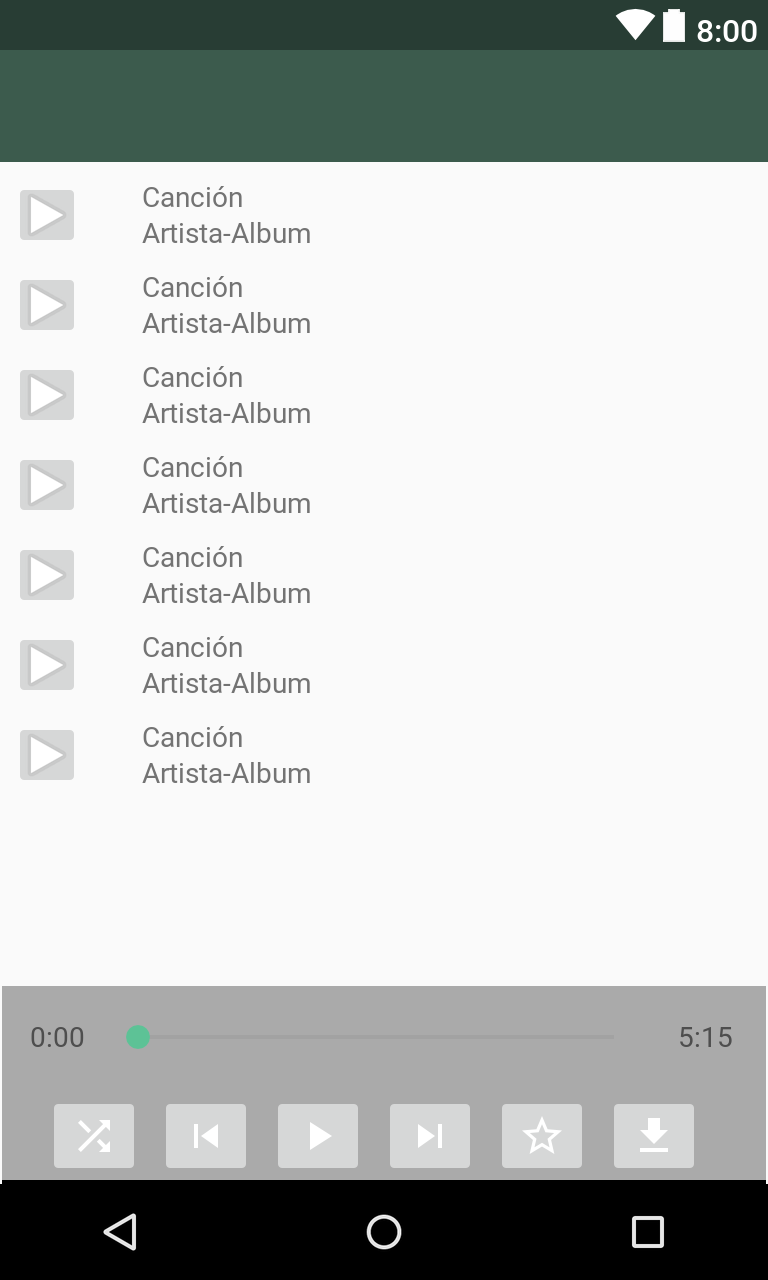
\includegraphics[width=6cm]{Figures/android/lista-reproductor.png} \\
\hline
\\
La forma de ir de una pantalla a otra en la aplicación sería mediante un panel lateral.
&
Desde cualquier pantalla se puede reproducir música, no es necesario que se esté en la pantalla del reproductor \\
\hline
\end{tabular}

\begin{tabular}{ p{6cm} p{6cm}}
\hline
\\
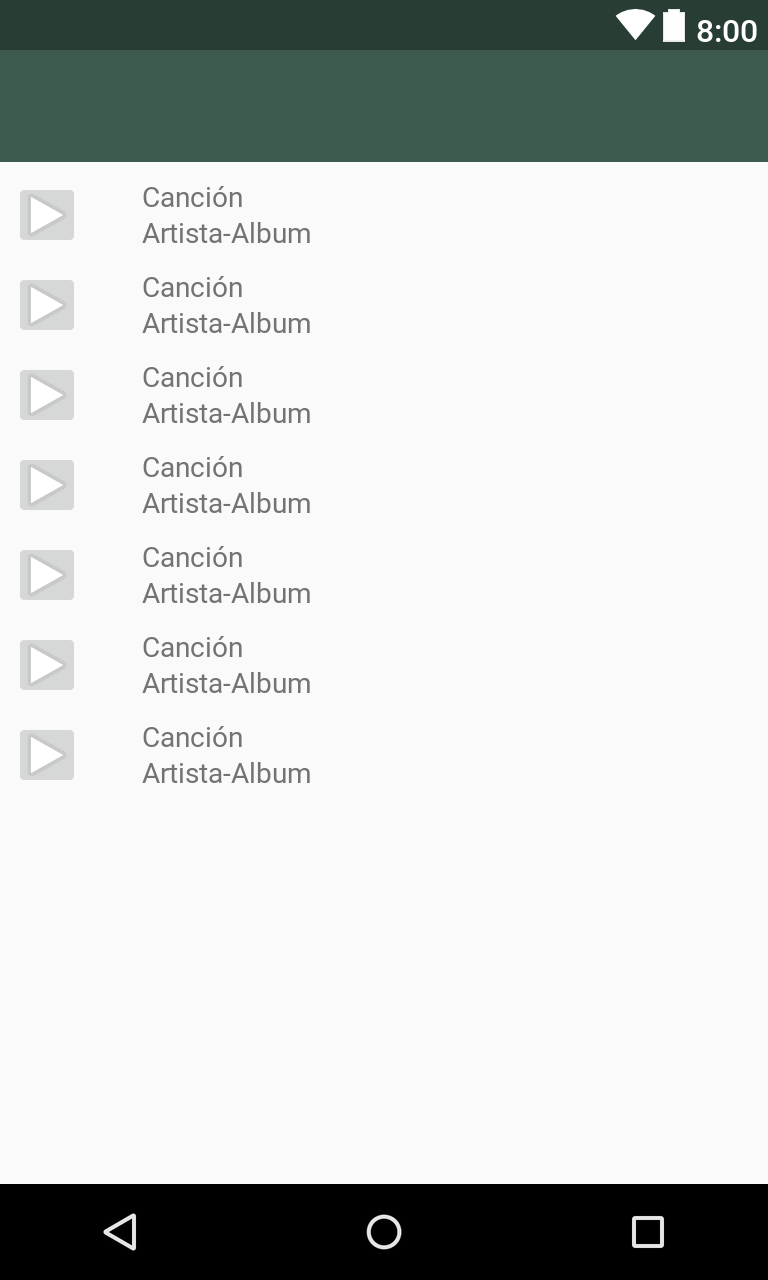
\includegraphics[width=6cm]{Figures/android/lista-no-personal.png}
&
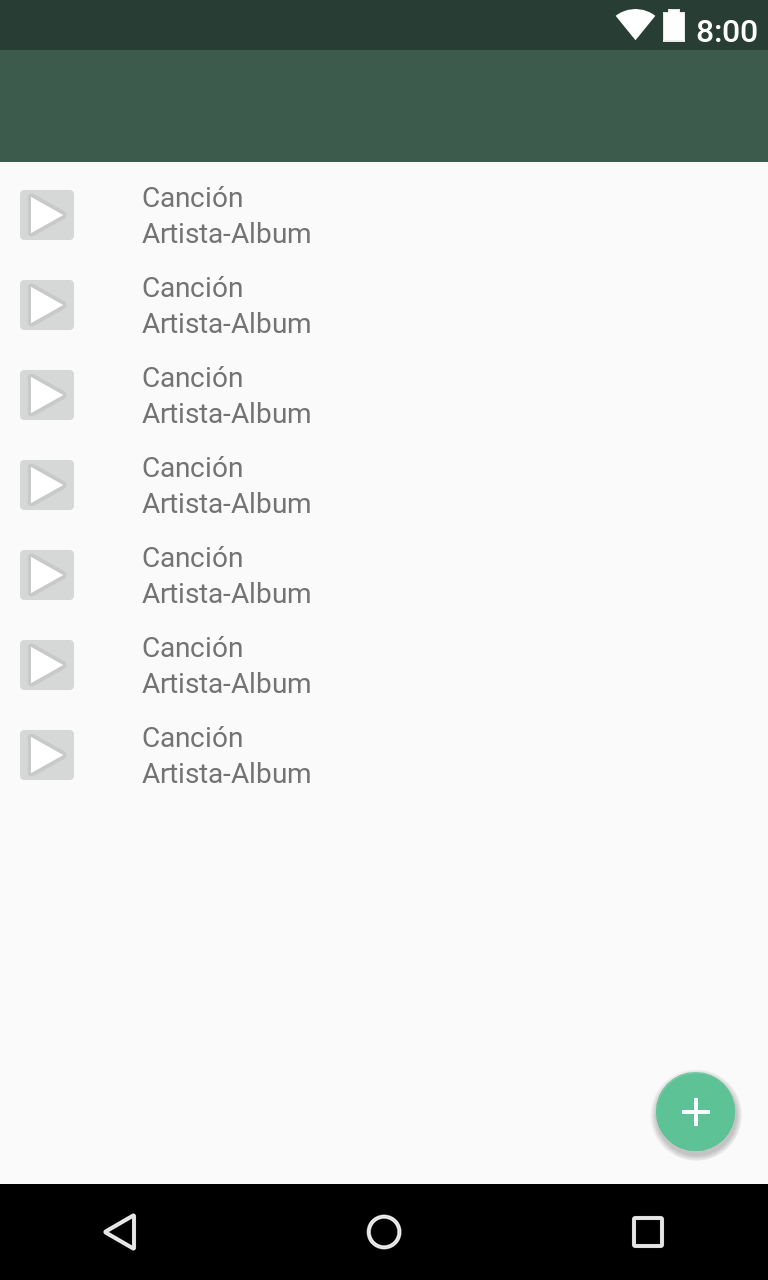
\includegraphics[width=6cm]{Figures/android/lista-personal.png} \\
\hline
\\
Lista de canciones, artistas o playlists. Este esquema de pantalla sería el que se produce al realizar una búsqueda o al acceder a las distintas categorías de mi biblioteca (playlist a las que sigues, canciones que te han gustado, artistas a los que sigues y canciones descargadas).
&
Este esquema de pantalla sería el que se produce al acceder a “Mis canciones” o “Mis playlists”.
Difiere del anterior en que permite añadir más elementos desde la pantalla. \\
\hline
\end{tabular}

\begin{tabular}{ p{6cm} p{6cm}}
\hline
\\
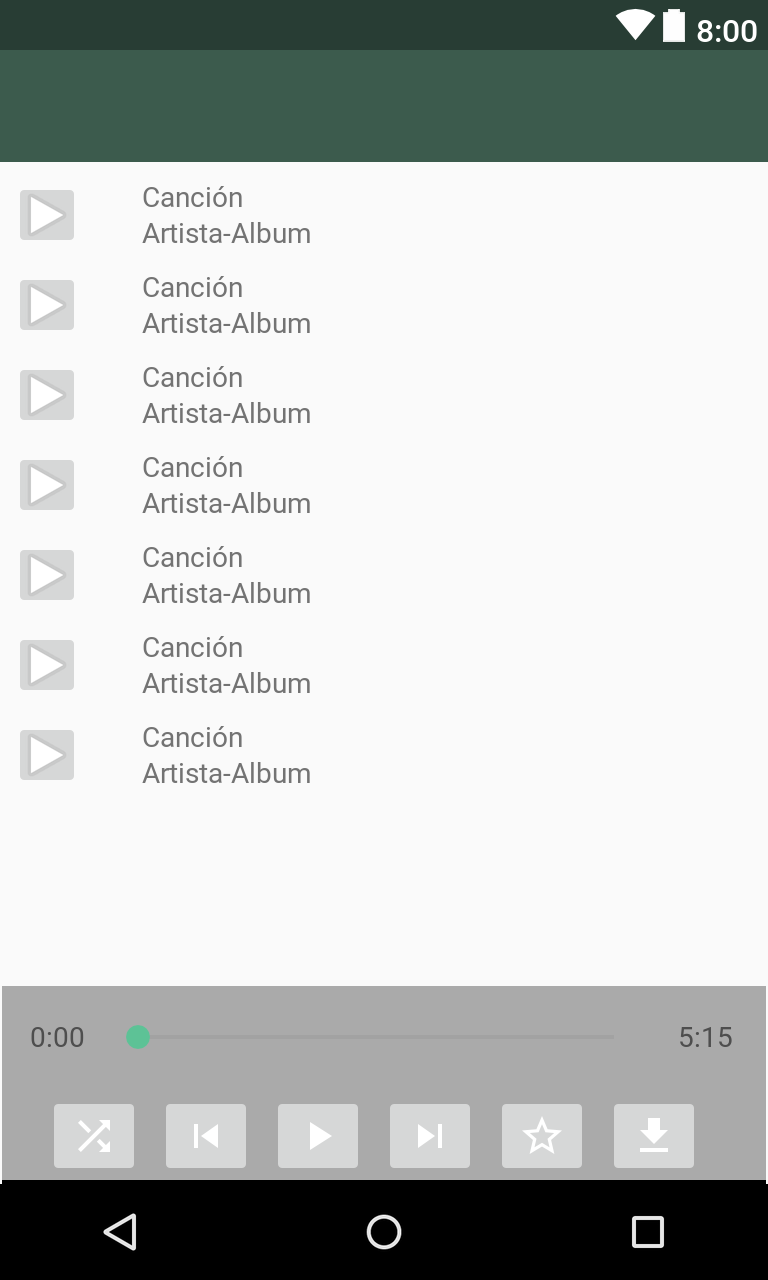
\includegraphics[width=6cm]{Figures/android/lista-reproductor.png}
&
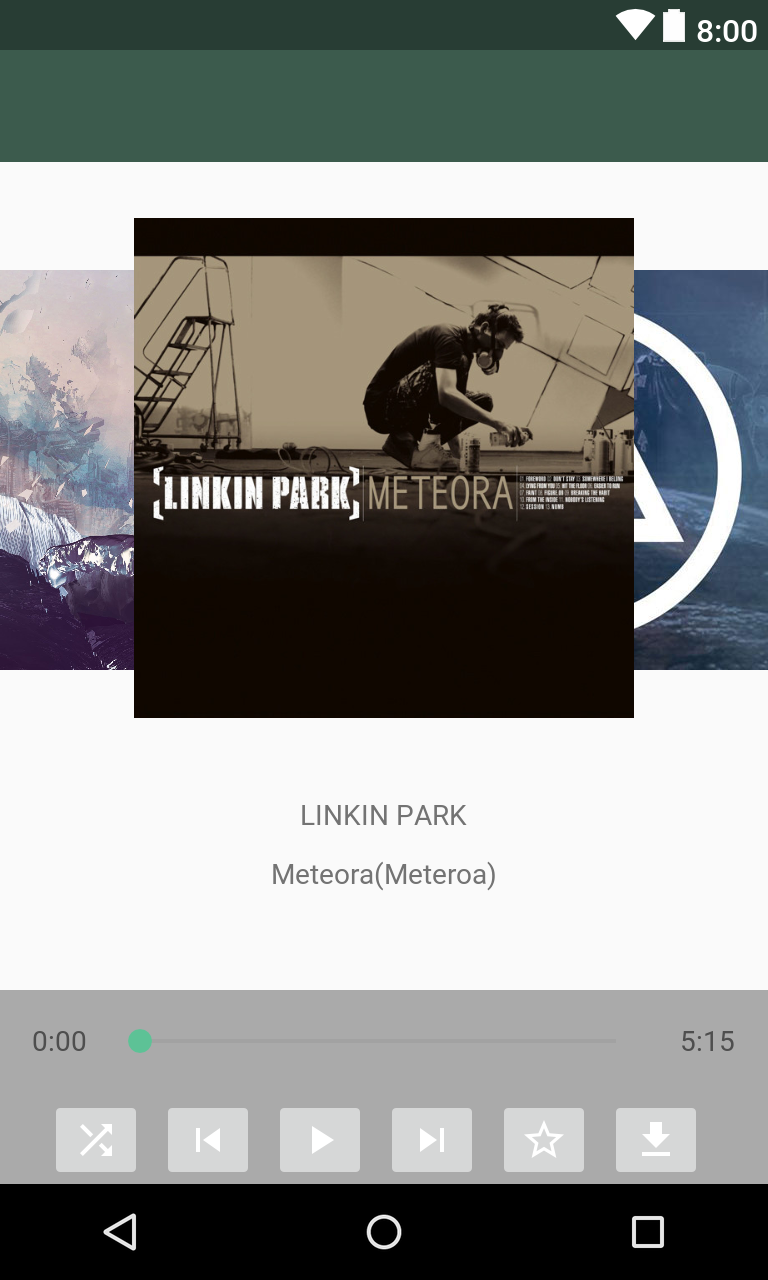
\includegraphics[width=6cm]{Figures/android/Reproductor.png} \\
\hline
\\
Desde cualquier pantalla se puede reproducir música, no es necesario que se esté en la pantalla del reproductor, en este caso se está reproduciendo desde una lista de canciones.
&
Pantalla del reproductor de música desde la que de puede descargar una canción, añadirla a favoritos ( opción de “me gusta”) . Desde esta pantalla también se podría compartirla en redes sociales. 
Esta pantalla se abre cuando se pulsa sobre una canción. \\
\hline
\end{tabular}

\begin{tabular}{ p{6cm} p{6cm}}
\hline
\\
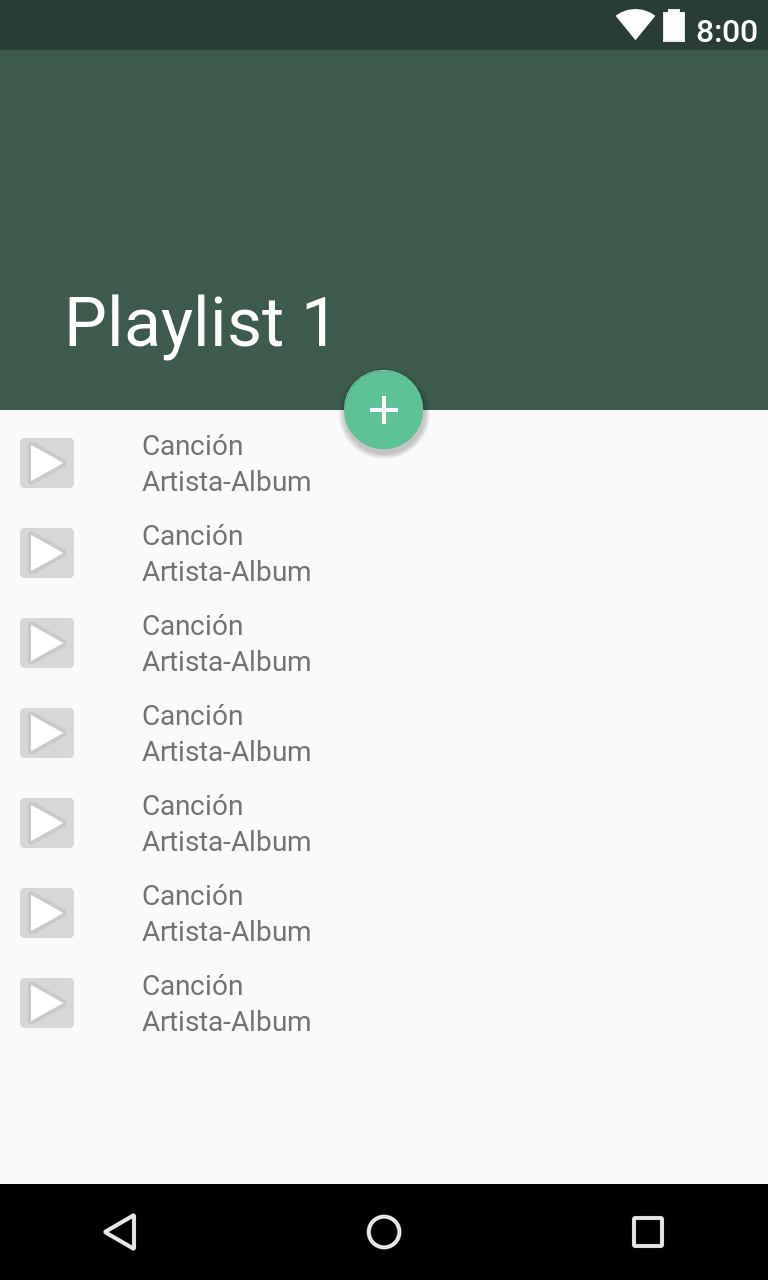
\includegraphics[width=6cm]{Figures/android/PlayList.png}
&
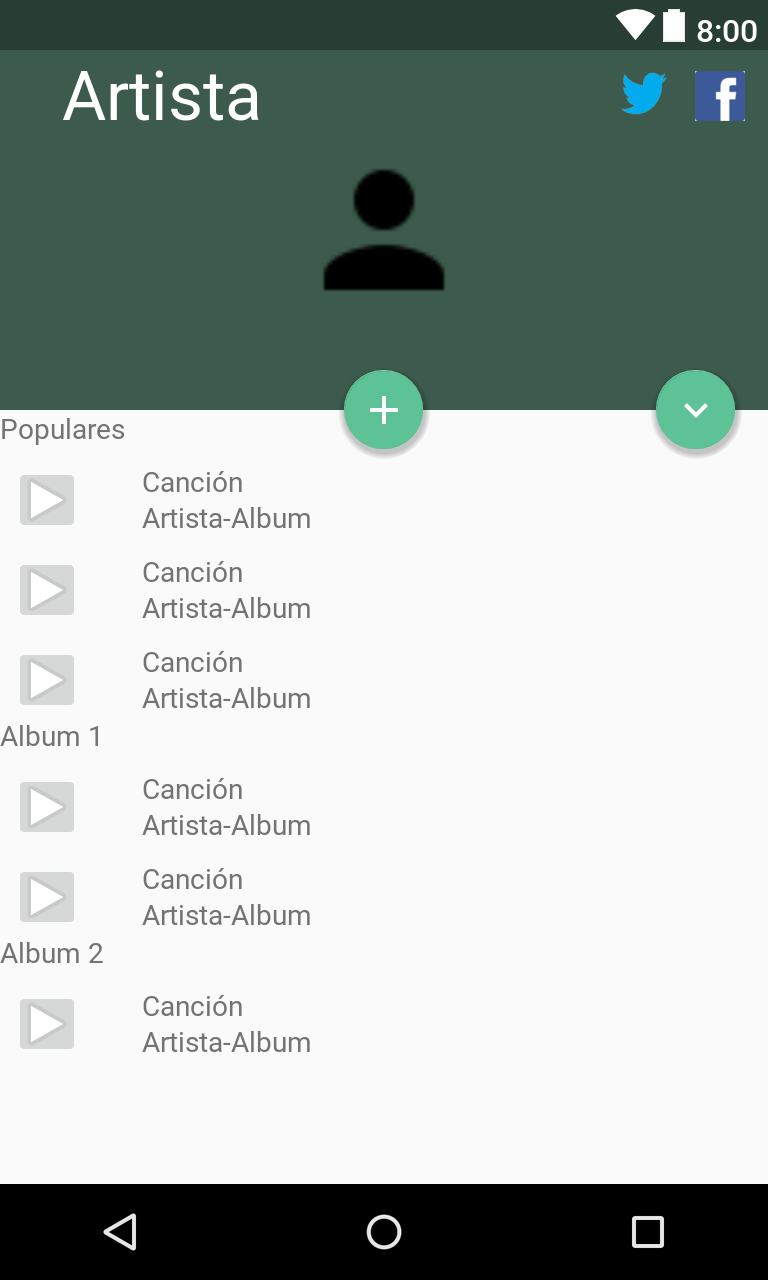
\includegraphics[width=6cm]{Figures/android/artista.png} \\
\hline
\\
Pantalla que aparece al pulsar sobre una playlist, desde la que se pueden ver las canciones que hay en dicha lista de reproducción, el creador de esta, así como suscribirse a ella.
&
Pantalla de perfil de usuario (perfil de artista), en la cual aparecen las canciones de un usuario clasificadas por álbumes, así como las listas de reproducción creadas por este usuario. También aparecen enlaces con redes sociales y la posibilidad de suscribirte a este usuario.
En esta pantalla también aparecerían estadísticas del usuario como pueden ser numero de seguidores o el número de visitas o “me gusta” que poseen sus canciones.  
\\
\hline
\end{tabular}
% ______________________
% Aqui termina la tabla

\vspace{1cm}
Las pantallas relacionadas con la subida de canciones y registro de usuario no se han incluido debido a que serían formularios.
La pantalla mi perfil no se ha incluido, aunque esta estaría compuesta por la información personal así como estadísticas de la cuenta (número de reproducciones totales recibidos, número de me gusta totales recibidos). También se daría la opción de editar la información personal.

\subsection{Prototipo pantallas Web}

\begin{tabular}{ p{6cm} p{6cm}}
	\hline
	\\
	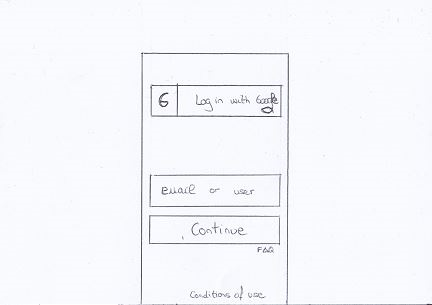
\includegraphics[width=6cm]{Figures/web/Login-web.png}
	&
	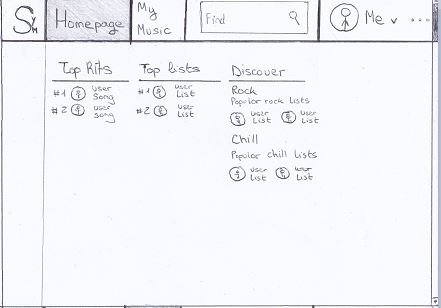
\includegraphics[width=6cm]{Figures/web/Lista-web.png} \\
	\hline
	\\
	Esta pantalla corresponde al inicio de sesión en la web y si es nuevo usuario, al registro del mismo.
	Se puede acceder mediante cuenta propia de la aplicación web (email o usuario) o mediante una cuenta de Google Plus.
	&
	Esta pantalla correspondería con la ventana principal en la aplicación, a traves de la cual se puede revisar la mejor música del momento recomendada para el usuario o acceder al resto de opciones (colección de álbunes, listas o pistas personales, búsquedas personalizadas o el propio perfil del usuario y su configuración).
	La aplicación permite al usuario reproducir la pista que desee haciendo click en sobre esta misma, procediendo así la aplicacíon a abrir en la parte inferior de la ventana la información de la pista y su estado actual (segundo de reproducción, si el usuario la ha marcado como favorita, etcétera).
	\\
	\hline
\end{tabular}

\begin{tabular}{ p{6cm} p{6cm}}
	\hline
	\\
	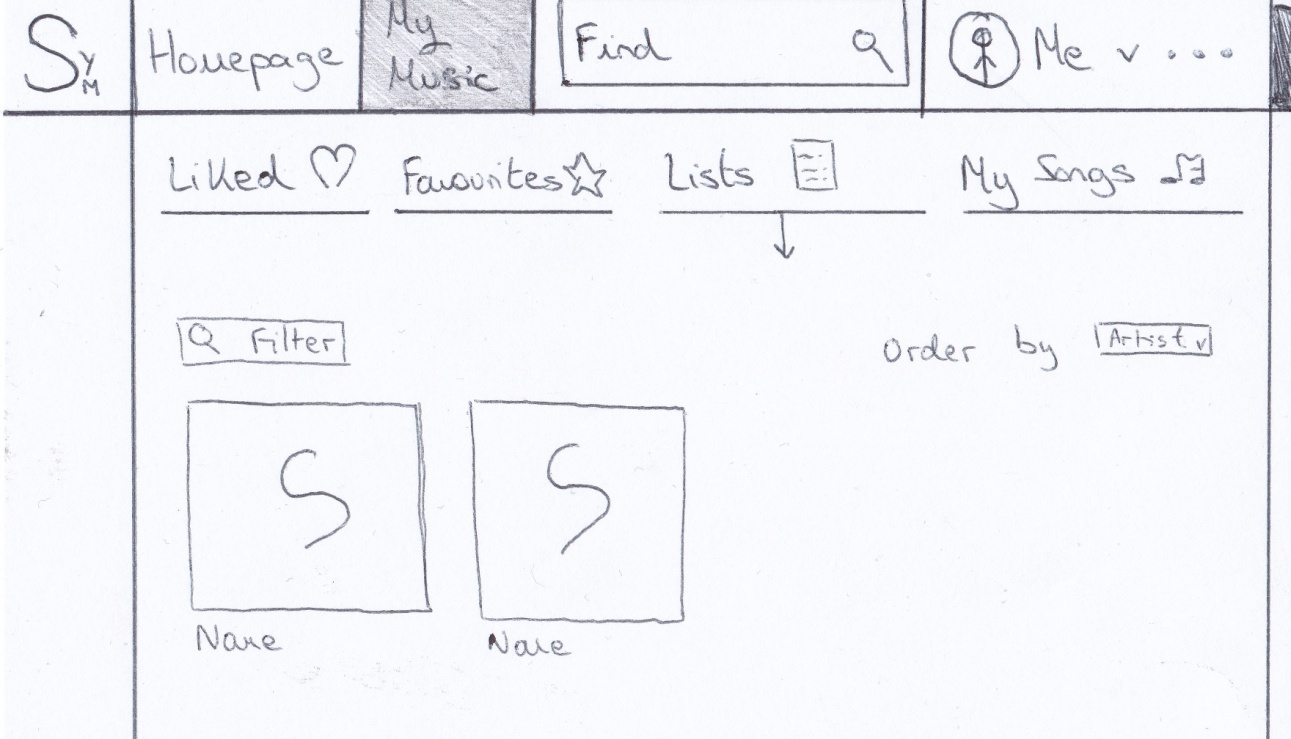
\includegraphics[width=6cm]{Figures/web/Main-web.png}
	&
	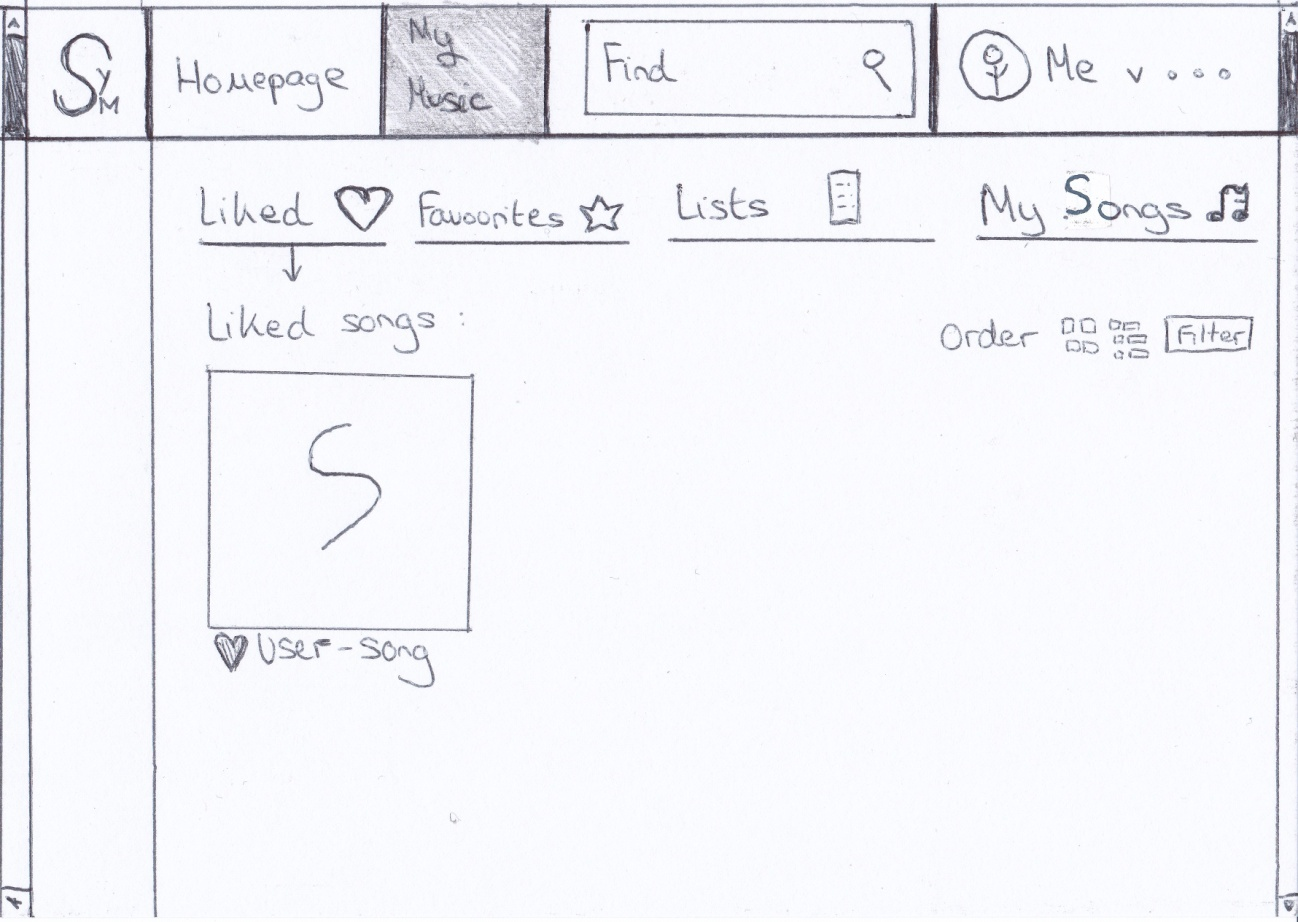
\includegraphics[width=6cm]{Figures/web/Reproduction-web.png} \\
	\hline
	\\
	Esta pantalla correspondería con tu colección de música en la aplicación, a traves de la cual se puede revisar la colección de álbunes, listas o pistas personales, así como las canciones que le gustan al usuario y sus canciones favoritas, ordenarlas o filtrarlas de manera personalizada.
	En este caso el usuario vería sus listas personales.
	La aplicación permite al usuario reproducir la pista que desee haciendo click en sobre esta misma, procediendo así la aplicacíon a abrir en la parte inferior de la ventana la información de la pista y su estado actual (segundo de reproducción, si el usuario la ha marcado como favorita, etcétera).
	&
	Esta pantalla correspondería con tu colección de música en la aplicación, donde a diferencia  de la anterior el usuario ha seleccionado visualizar las canciones que le gustan.
	La aplicación permite al usuario reproducir la pista que desee haciendo click en sobre esta misma, procediendo así la aplicacíon a abrir en la parte inferior de la ventana la información de la pista y su estado actual (segundo de reproducción, si el usuario la ha marcado como favorita, etcétera).
	\\
	\hline
\end{tabular}

\begin{tabular}{ p{6cm} p{6cm}}
	\hline
	\\
	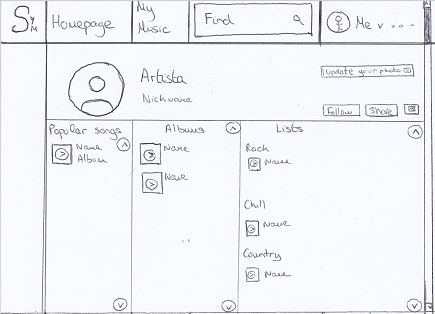
\includegraphics[width=6cm]{Figures/web/Artist-web.png}
	&
	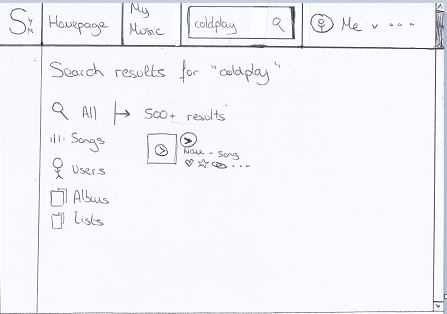
\includegraphics[width=6cm]{Figures/web/search-web.png} \\
	\hline
	\\
	Esta pantalla se correspondería con la vista general de un usuario donde este puede editar su foto de perfil si es el dueño de la cuenta o si es otro usuario suscribirse a las listas/pistas del usuario deseado.
	Se puede realizar scroll tanto en las canciones como listas o albunes del usuario.
	La aplicación permite al usuario reproducir la pista que desee haciendo click en sobre esta misma, procediendo así la aplicacíon a abrir en la parte inferior de la ventana la información de la pista y su estado actual (segundo de reproducción, si el usuario la ha marcado como favorita, etcétera).
	&
	Esta pantalla se correspondería con la obtención de resultados tras la búsqueda personalizada de un usuario que desea que le muestren toda la información disponible a cerca de las palabras clave seleccionadas, también se podría filtrar por pistas, listas, albunes o artistas disponibles.
	La aplicación permite al usuario reproducir la pista que desee haciendo click en sobre esta misma, procediendo así la aplicacíon a abrir en la parte inferior de la ventana la información de la pista y su estado actual (segundo de reproducción, si el usuario la ha marcado como favorita, etcétera).
	\\
	\hline
\end{tabular} 
% Chapter Template

\chapter{Descripci\'on t\'ecnica} % Main chapter title

\label{Chapter3} % Change X to a consecutive number; for referencing this chapter elsewhere, use \ref{ChapterX}

%----------------------------------------------------------------------------------------
%	SECTION 1
%----------------------------------------------------------------------------------------

\section{Descripci\'on t\'ecnica}

\begin{itemize}
	\item Aspectos técnicos de relevancia para los usuarios: por ejemplo, que el sistema requiera al menos cierta versión de Android o iOS es relevante para los usuarios. Que se va a usar PostgreSQL versión 9.2 no lo es.

	\item Aspectos técnicos de relevancia para los clientes: por ejemplo, que el sistema se va a entregar instalado en un servidor virtual desplegado en AWS es relevante para los clientes (que tendrán que seguir pagando la cuota mensual para seguir funcionando). También lo es si se va a entregar o no el código fuente, si se va a poder desplegar on premises (en un centro de datos del propio cliente) y si es así que Sistema Operativo va a requerir etc.
	
	\item Descripción técnica preliminar de la solución a desarrollar. Principales componentes tecnológicos, cómo se conectan entre sí, qué hardware requieren para su despliegue. El objetivo de este punto es convencer de que la propuesta que se está haciendo es técnicamente sólida, y que el proveedor sabe de lo que habla. No es el diseño arquitectural detallado que el proveedor tendrá que hacer internamente.
\end{itemize}

% Chapter Template

\chapter{Análisis y diseño del sistema} % Main chapter title

\label{Chapter4} % Change X to a consecutive number; for referencing this chapter elsewhere, use \ref{ChapterX}

\section{Análisis de requisitos}
Completar y detallar los requisitos preliminares incluidos en la propuesta técnica y económica. Recordad que los requisitos deben ser completos, concretos, medibles cuando tenga sentido y lo menos ambiguos posible. También es importante que estén identificados para facilitar su trazabilidad.

\section{Diseño del sistema}
\begin{itemize}
	\item Diagramas arquitecturales (de módulos, de componentes y conectores, de distribución), patrones de diseño y estilos arquitecturales que se aplicarán. Las interfaces (de módulos y de componentes) son especialmente importantes. También lo son los protocolos de comunicación entre componentes.
	\item Tecnologías elegidas (lenguajes de programación, componentes que se integrarán, API web externas con las que se conectará etc.).
	\item Otros aspectos técnicos de interés (p.ej. si hay base de datos si va a ser SQL o NoSQL, si hay una API Web va a ser RESTful o no, si algunas de las operaciones van a ser asíncronas o no, si va a ser una aplicación móvil o de escritorio será nativa o se van a usar tecnologías web, cómo se van a considerar los requisitos de seguridad o de prestaciones, cómo y dónde se harán las instalaciones y despliegues etc.)
\end{itemize}

Hay que justificar todas las decisiones de diseño. Esto exige contestar a dos preguntas sobre cada decisión: ¿qué alternativas se barajaron? y ¿por qué se eligió una y no las otras?
 
% Chapter Template

\chapter{Memoria del proyecto} % Main chapter title

\label{Chapter5} % Change X to a consecutive number; for referencing this chapter elsewhere, use \ref{ChapterX}


ESTE CAPÍTULO NO SE RELLENA EN LA PRIMERA ENTREGA
En este capítulo se describirá cómo se ha llevado a cabo el proyecto, qué cambios se han hecho respecto a la versión inicial, imprevistos surgidos, etc.
\section{Inicio del proyecto}
Describir cómo transcurrió esta fase del proyecto, especialmente los resultados de llevar a cabo los procesos descritos en la sección Procesos de inicio del proyecto.
\section{Ejecución y control del proyecto}
Describir cómo transcurrió esta fase del proyecto, especialmente los resultados de llevar a cabo los procesos descritos en la sección Procesos de ejecución y control del proyecto y en la sección Procesos técnicos. No olvidar:
\begin{itemize}
	\item Cómo se ha realizado el reparto de trabajo entre miembros del equipo. Cómo ha transcurrido la comunicación interna.
	\item Cómo se ha medido el progreso del proyecto. Cómo se sabía el trabajo realizado, el trabajo pendiente y lo que estaba haciendo cada persona.
	\item Los ajustes realizados cuando se detectaron divergencias frente al calendario inicial (ajustes en el trabajo y/o ajustes en el calendario). Si se han identificado las causas de estas divergencias, explicarlas.
	\item Adecuación de las herramientas y tecnologías empleadas. Si ha habido que cambiar alguna decisión de diseño o de tecnología, y por qué.
	\item Funcionamiento de los procesos de control de versiones del código, construcción y despliegue. ¿Ha habido problemas con las integraciones? ¿Problemas con los despliegues? ¿Se han perdido cosas por errores humanos? ¿Cómo se han abordado estas tareas?
	\item Pruebas del software. ¿Se han podido cumplir las ideas que se tenían al respecto?
\end{itemize}

\section{Cierre del proyecto}
Al menos:
\begin{itemize}
	\item Comparar las estimaciones iniciales (tamaño, esfuerzos, costes) con los resultados finales, analizar los resultados y tratar de expresar algunas lecciones aprendidas.
	\item Lecciones aprendidas sobre herramientas y tecnologías.
	\item Recopilar los esfuerzos dedicados al proyecto por cada uno de los participantes: horas trabajadas y actividades realizadas por cada persona.
\end{itemize} 
% Chapter Template

\chapter{Conclusiones} % Main chapter title

\label{Chapter6} % Change X to a consecutive number; for referencing this chapter elsewhere, use \ref{ChapterX}

%----------------------------------------------------------------------------------------
%	SECTION 1
%----------------------------------------------------------------------------------------


ESTE CAPÍTULO SOLO SE RELLENA EN LA ENTREGA FINAL
Además de conclusiones personales (razonadas) sobre el transcurso del proyecto realizado, es importante plantear ideas para mejorar los procesos llevados a cabo: si hubiera que iniciar un nuevo proyecto inmediatamente usando una metodología de gestión basada en procesos, ¿qué cambios haríais respecto a los procesos que habéis seguido durante este proyecto?  ¿Qué cosas está claro que haríais de otra forma? ¿Qué cosas seguiríais haciendo más o menos igual?


%----------------------------------------------------------------------------------------
%	THESIS CONTENT - APPENDICES
%----------------------------------------------------------------------------------------

\appendix % Cue to tell LaTeX that the following "chapters" are Appendices

% Include the appendices of the thesis as separate files from the Appendices folder
% Uncomment the lines as you write the Appendices

%% Appendix A

\chapter{Dedicaci\'on} % Main appendix title

\label{AppendixA} % For referencing this appendix elsewhere, use \ref{AppendixA}

\section{Dedicaci\'on}

\begin{table}[htbp]
	\caption{Dedicación a la práctica de los integrantes del grupo.}
	\label{tab:dedication}
	\centering
	\begin{tabular}{l l p{4in}}
		\toprule
		\tabhead{Integrante} & \tabhead{Dedicación (h)} & \tabhead{Partes desarrolladas} \\
		\midrule
		\'Angel Cañal & 40 & 
		\begin{itemize}
			\item A
		\end{itemize}\\
		Abel Chils & 40 & 
		\begin{itemize}
			\item A
		\end{itemize}\\
		Jorge Aznar & 40 & 
		\begin{itemize}
			\item A
		\end{itemize}\\
		Yasmina Albero & 40 & 
		\begin{itemize}
			\item A
		\end{itemize}\\
		\'Oscar Fraca & 40 & 
		\begin{itemize}
			\item A
		\end{itemize}\\
		Alexandru Oarga & 40 & 
		\begin{itemize}
			\item A
		\end{itemize}\\
		Jorge Pinilla & 40 & 
		\begin{itemize}
			\item B
		\end{itemize}\\
		\textit{Ambos} & --- & 
		\begin{itemize}
			\item Diagramas de secuencia de dise\~no pr\'acticas
		\end{itemize}\\
		\bottomrule\\
	\end{tabular}
\end{table}

\vfill



%\include{Appendices/AppendixB}
%\include{Appendices/AppendixC}

%----------------------------------------------------------------------------------------
%	BIBLIOGRAPHY
%----------------------------------------------------------------------------------------

\printbibliography[heading=bibintoc]

%----------------------------------------------------------------------------------------

\end{document}  
